% Created by tikzDevice version 0.12.5 on 2023-10-14 23:56:52
% !TEX encoding = UTF-8 Unicode
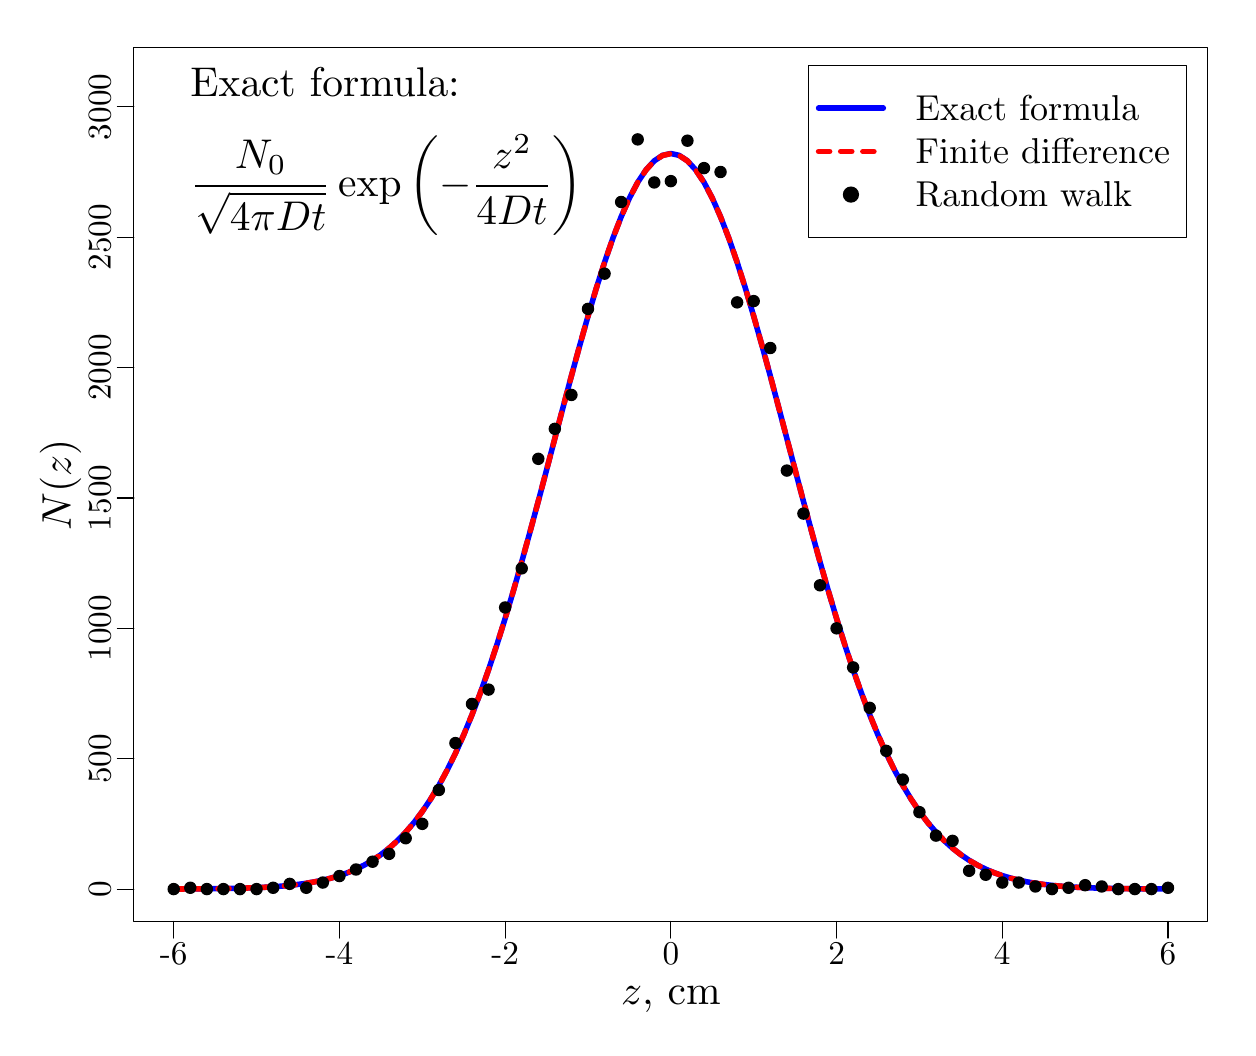
\begin{tikzpicture}[x=1pt,y=1pt]
\definecolor{fillColor}{RGB}{255,255,255}
\path[use as bounding box,fill=fillColor,fill opacity=0.00] (0,0) rectangle (433.62,361.35);
\begin{scope}
\path[clip] ( 38.40, 38.40) rectangle (426.42,354.15);
\definecolor{drawColor}{RGB}{0,0,255}

\path[draw=drawColor,line width= 2.0pt,line join=round,line cap=round] ( 52.77, 50.11) --
	( 55.77, 50.12) --
	( 58.76, 50.14) --
	( 61.75, 50.16) --
	( 64.75, 50.18) --
	( 67.74, 50.22) --
	( 70.73, 50.26) --
	( 73.73, 50.32) --
	( 76.72, 50.39) --
	( 79.72, 50.48) --
	( 82.71, 50.59) --
	( 85.70, 50.74) --
	( 88.70, 50.92) --
	( 91.69, 51.14) --
	( 94.69, 51.42) --
	( 97.68, 51.76) --
	(100.67, 52.18) --
	(103.67, 52.69) --
	(106.66, 53.31) --
	(109.66, 54.06) --
	(112.65, 54.95) --
	(115.64, 56.01) --
	(118.64, 57.27) --
	(121.63, 58.75) --
	(124.63, 60.49) --
	(127.62, 62.51) --
	(130.61, 64.85) --
	(133.61, 67.55) --
	(136.60, 70.63) --
	(139.60, 74.13) --
	(142.59, 78.09) --
	(145.58, 82.55) --
	(148.58, 87.52) --
	(151.57, 93.04) --
	(154.57, 99.12) --
	(157.56,105.79) --
	(160.55,113.05) --
	(163.55,120.91) --
	(166.54,129.34) --
	(169.54,138.34) --
	(172.53,147.86) --
	(175.52,157.88) --
	(178.52,168.32) --
	(181.51,179.13) --
	(184.51,190.23) --
	(187.50,201.53) --
	(190.49,212.91) --
	(193.49,224.29) --
	(196.48,235.52) --
	(199.48,246.50) --
	(202.47,257.08) --
	(205.46,267.15) --
	(208.46,276.58) --
	(211.45,285.23) --
	(214.45,293.00) --
	(217.44,299.77) --
	(220.43,305.46) --
	(223.43,309.96) --
	(226.42,313.23) --
	(229.42,315.21) --
	(232.41,315.88) --
	(235.40,315.21) --
	(238.40,313.23) --
	(241.39,309.96) --
	(244.39,305.46) --
	(247.38,299.77) --
	(250.37,293.00) --
	(253.37,285.23) --
	(256.36,276.58) --
	(259.36,267.15) --
	(262.35,257.08) --
	(265.34,246.50) --
	(268.34,235.52) --
	(271.33,224.29) --
	(274.33,212.91) --
	(277.32,201.53) --
	(280.31,190.23) --
	(283.31,179.13) --
	(286.30,168.32) --
	(289.30,157.88) --
	(292.29,147.86) --
	(295.28,138.34) --
	(298.28,129.34) --
	(301.27,120.91) --
	(304.27,113.05) --
	(307.26,105.79) --
	(310.25, 99.12) --
	(313.25, 93.04) --
	(316.24, 87.52) --
	(319.24, 82.55) --
	(322.23, 78.09) --
	(325.22, 74.13) --
	(328.22, 70.63) --
	(331.21, 67.55) --
	(334.21, 64.85) --
	(337.20, 62.51) --
	(340.19, 60.49) --
	(343.19, 58.75) --
	(346.18, 57.27) --
	(349.18, 56.01) --
	(352.17, 54.95) --
	(355.16, 54.06) --
	(358.16, 53.31) --
	(361.15, 52.69) --
	(364.15, 52.18) --
	(367.14, 51.76) --
	(370.13, 51.42) --
	(373.13, 51.14) --
	(376.12, 50.92) --
	(379.12, 50.74) --
	(382.11, 50.59) --
	(385.10, 50.48) --
	(388.10, 50.39) --
	(391.09, 50.32) --
	(394.08, 50.26) --
	(397.08, 50.22) --
	(400.07, 50.18) --
	(403.07, 50.16) --
	(406.06, 50.14) --
	(409.05, 50.12) --
	(412.05, 50.11);
\end{scope}
\begin{scope}
\path[clip] (  0.00,  0.00) rectangle (433.62,361.35);
\definecolor{drawColor}{RGB}{0,0,0}

\path[draw=drawColor,line width= 0.4pt,line join=round,line cap=round] ( 52.77, 38.40) -- (412.05, 38.40);

\path[draw=drawColor,line width= 0.4pt,line join=round,line cap=round] ( 52.77, 38.40) -- ( 52.77, 32.40);

\path[draw=drawColor,line width= 0.4pt,line join=round,line cap=round] (112.65, 38.40) -- (112.65, 32.40);

\path[draw=drawColor,line width= 0.4pt,line join=round,line cap=round] (172.53, 38.40) -- (172.53, 32.40);

\path[draw=drawColor,line width= 0.4pt,line join=round,line cap=round] (232.41, 38.40) -- (232.41, 32.40);

\path[draw=drawColor,line width= 0.4pt,line join=round,line cap=round] (292.29, 38.40) -- (292.29, 32.40);

\path[draw=drawColor,line width= 0.4pt,line join=round,line cap=round] (352.17, 38.40) -- (352.17, 32.40);

\path[draw=drawColor,line width= 0.4pt,line join=round,line cap=round] (412.05, 38.40) -- (412.05, 32.40);

\node[text=drawColor,anchor=base,inner sep=0pt, outer sep=0pt, scale=  1.20] at ( 52.77, 22.80) {-6};

\node[text=drawColor,anchor=base,inner sep=0pt, outer sep=0pt, scale=  1.20] at (112.65, 22.80) {-4};

\node[text=drawColor,anchor=base,inner sep=0pt, outer sep=0pt, scale=  1.20] at (172.53, 22.80) {-2};

\node[text=drawColor,anchor=base,inner sep=0pt, outer sep=0pt, scale=  1.20] at (232.41, 22.80) {0};

\node[text=drawColor,anchor=base,inner sep=0pt, outer sep=0pt, scale=  1.20] at (292.29, 22.80) {2};

\node[text=drawColor,anchor=base,inner sep=0pt, outer sep=0pt, scale=  1.20] at (352.17, 22.80) {4};

\node[text=drawColor,anchor=base,inner sep=0pt, outer sep=0pt, scale=  1.20] at (412.05, 22.80) {6};

\path[draw=drawColor,line width= 0.4pt,line join=round,line cap=round] ( 38.40, 50.08) -- ( 38.40,332.75);

\path[draw=drawColor,line width= 0.4pt,line join=round,line cap=round] ( 38.40, 50.08) -- ( 32.40, 50.08);

\path[draw=drawColor,line width= 0.4pt,line join=round,line cap=round] ( 38.40, 97.19) -- ( 32.40, 97.19);

\path[draw=drawColor,line width= 0.4pt,line join=round,line cap=round] ( 38.40,144.30) -- ( 32.40,144.30);

\path[draw=drawColor,line width= 0.4pt,line join=round,line cap=round] ( 38.40,191.41) -- ( 32.40,191.41);

\path[draw=drawColor,line width= 0.4pt,line join=round,line cap=round] ( 38.40,238.53) -- ( 32.40,238.53);

\path[draw=drawColor,line width= 0.4pt,line join=round,line cap=round] ( 38.40,285.64) -- ( 32.40,285.64);

\path[draw=drawColor,line width= 0.4pt,line join=round,line cap=round] ( 38.40,332.75) -- ( 32.40,332.75);

\node[text=drawColor,rotate= 90.00,anchor=base,inner sep=0pt, outer sep=0pt, scale=  1.20] at ( 30.00, 50.08) {0};

\node[text=drawColor,rotate= 90.00,anchor=base,inner sep=0pt, outer sep=0pt, scale=  1.20] at ( 30.00, 97.19) {500};

\node[text=drawColor,rotate= 90.00,anchor=base,inner sep=0pt, outer sep=0pt, scale=  1.20] at ( 30.00,144.30) {1000};

\node[text=drawColor,rotate= 90.00,anchor=base,inner sep=0pt, outer sep=0pt, scale=  1.20] at ( 30.00,191.41) {1500};

\node[text=drawColor,rotate= 90.00,anchor=base,inner sep=0pt, outer sep=0pt, scale=  1.20] at ( 30.00,238.53) {2000};

\node[text=drawColor,rotate= 90.00,anchor=base,inner sep=0pt, outer sep=0pt, scale=  1.20] at ( 30.00,285.64) {2500};

\node[text=drawColor,rotate= 90.00,anchor=base,inner sep=0pt, outer sep=0pt, scale=  1.20] at ( 30.00,332.75) {3000};

\path[draw=drawColor,line width= 0.4pt,line join=round,line cap=round] ( 38.40, 38.40) --
	(426.42, 38.40) --
	(426.42,354.15) --
	( 38.40,354.15) --
	cycle;
\end{scope}
\begin{scope}
\path[clip] (  0.00,  0.00) rectangle (433.62,361.35);
\definecolor{drawColor}{RGB}{0,0,0}

\node[text=drawColor,anchor=base,inner sep=0pt, outer sep=0pt, scale=  1.50] at (232.41,  8.40) {$z$, cm};

\node[text=drawColor,rotate= 90.00,anchor=base,inner sep=0pt, outer sep=0pt, scale=  1.50] at ( 15.60,196.27) {$N(z)$};
\end{scope}
\begin{scope}
\path[clip] ( 38.40, 38.40) rectangle (426.42,354.15);
\definecolor{drawColor}{RGB}{255,0,0}

\path[draw=drawColor,line width= 2.0pt,dash pattern=on 4pt off 4pt ,line join=round,line cap=round] ( 52.77, 50.09) --
	( 55.77, 50.11) --
	( 58.76, 50.13) --
	( 61.75, 50.15) --
	( 64.75, 50.18) --
	( 67.74, 50.21) --
	( 70.73, 50.26) --
	( 73.73, 50.31) --
	( 76.72, 50.39) --
	( 79.72, 50.48) --
	( 82.71, 50.59) --
	( 85.70, 50.73) --
	( 88.70, 50.91) --
	( 91.69, 51.14) --
	( 94.69, 51.42) --
	( 97.68, 51.76) --
	(100.67, 52.18) --
	(103.67, 52.69) --
	(106.66, 53.31) --
	(109.66, 54.05) --
	(112.65, 54.94) --
	(115.64, 56.01) --
	(118.64, 57.27) --
	(121.63, 58.75) --
	(124.63, 60.49) --
	(127.62, 62.51) --
	(130.61, 64.85) --
	(133.61, 67.55) --
	(136.60, 70.63) --
	(139.60, 74.13) --
	(142.59, 78.10) --
	(145.58, 82.55) --
	(148.58, 87.53) --
	(151.57, 93.05) --
	(154.57, 99.14) --
	(157.56,105.81) --
	(160.55,113.07) --
	(163.55,120.92) --
	(166.54,129.36) --
	(169.54,138.35) --
	(172.53,147.88) --
	(175.52,157.90) --
	(178.52,168.34) --
	(181.51,179.15) --
	(184.51,190.25) --
	(187.50,201.54) --
	(190.49,212.93) --
	(193.49,224.29) --
	(196.48,235.53) --
	(199.48,246.50) --
	(202.47,257.08) --
	(205.46,267.15) --
	(208.46,276.57) --
	(211.45,285.22) --
	(214.45,292.98) --
	(217.44,299.75) --
	(220.43,305.43) --
	(223.43,309.93) --
	(226.42,313.20) --
	(229.42,315.18) --
	(232.41,315.84) --
	(235.40,315.18) --
	(238.40,313.20) --
	(241.39,309.93) --
	(244.39,305.43) --
	(247.38,299.75) --
	(250.37,292.98) --
	(253.37,285.22) --
	(256.36,276.57) --
	(259.36,267.15) --
	(262.35,257.08) --
	(265.34,246.50) --
	(268.34,235.53) --
	(271.33,224.29) --
	(274.33,212.93) --
	(277.32,201.54) --
	(280.31,190.25) --
	(283.31,179.15) --
	(286.30,168.34) --
	(289.30,157.90) --
	(292.29,147.88) --
	(295.28,138.35) --
	(298.28,129.36) --
	(301.27,120.92) --
	(304.27,113.07) --
	(307.26,105.81) --
	(310.25, 99.14) --
	(313.25, 93.05) --
	(316.24, 87.53) --
	(319.24, 82.55) --
	(322.23, 78.10) --
	(325.22, 74.13) --
	(328.22, 70.63) --
	(331.21, 67.55) --
	(334.21, 64.85) --
	(337.20, 62.51) --
	(340.19, 60.49) --
	(343.19, 58.75) --
	(346.18, 57.27) --
	(349.18, 56.01) --
	(352.17, 54.94) --
	(355.16, 54.05) --
	(358.16, 53.31) --
	(361.15, 52.69) --
	(364.15, 52.18) --
	(367.14, 51.76) --
	(370.13, 51.42) --
	(373.13, 51.14) --
	(376.12, 50.91) --
	(379.12, 50.73) --
	(382.11, 50.59) --
	(385.10, 50.48) --
	(388.10, 50.39) --
	(391.09, 50.31) --
	(394.08, 50.26) --
	(397.08, 50.21) --
	(400.07, 50.18) --
	(403.07, 50.15) --
	(406.06, 50.13) --
	(409.05, 50.11) --
	(412.05, 50.09);
\definecolor{fillColor}{RGB}{0,0,0}

\path[fill=fillColor] ( 52.77, 50.08) circle (  2.25);

\path[fill=fillColor] ( 58.76, 50.55) circle (  2.25);

\path[fill=fillColor] ( 64.75, 50.08) circle (  2.25);

\path[fill=fillColor] ( 70.73, 50.08) circle (  2.25);

\path[fill=fillColor] ( 76.72, 50.08) circle (  2.25);

\path[fill=fillColor] ( 82.71, 50.08) circle (  2.25);

\path[fill=fillColor] ( 88.70, 50.55) circle (  2.25);

\path[fill=fillColor] ( 94.69, 51.96) circle (  2.25);

\path[fill=fillColor] (100.67, 50.55) circle (  2.25);

\path[fill=fillColor] (106.66, 52.44) circle (  2.25);

\path[fill=fillColor] (112.65, 54.79) circle (  2.25);

\path[fill=fillColor] (118.64, 57.15) circle (  2.25);

\path[fill=fillColor] (124.63, 59.97) circle (  2.25);

\path[fill=fillColor] (130.61, 62.80) circle (  2.25);

\path[fill=fillColor] (136.60, 68.45) circle (  2.25);

\path[fill=fillColor] (142.59, 73.64) circle (  2.25);

\path[fill=fillColor] (148.58, 85.88) circle (  2.25);

\path[fill=fillColor] (154.57,102.84) circle (  2.25);

\path[fill=fillColor] (160.55,116.98) circle (  2.25);

\path[fill=fillColor] (166.54,122.16) circle (  2.25);

\path[fill=fillColor] (172.53,151.84) circle (  2.25);

\path[fill=fillColor] (178.52,165.97) circle (  2.25);

\path[fill=fillColor] (184.51,205.55) circle (  2.25);

\path[fill=fillColor] (190.49,216.38) circle (  2.25);

\path[fill=fillColor] (196.48,228.63) circle (  2.25);

\path[fill=fillColor] (202.47,259.73) circle (  2.25);

\path[fill=fillColor] (208.46,272.45) circle (  2.25);

\path[fill=fillColor] (214.45,298.36) circle (  2.25);

\path[fill=fillColor] (220.43,320.97) circle (  2.25);

\path[fill=fillColor] (226.42,305.42) circle (  2.25);

\path[fill=fillColor] (232.41,305.89) circle (  2.25);

\path[fill=fillColor] (238.40,320.50) circle (  2.25);

\path[fill=fillColor] (244.39,310.61) circle (  2.25);

\path[fill=fillColor] (250.37,309.19) circle (  2.25);

\path[fill=fillColor] (256.36,262.08) circle (  2.25);

\path[fill=fillColor] (262.35,262.55) circle (  2.25);

\path[fill=fillColor] (268.34,245.59) circle (  2.25);

\path[fill=fillColor] (274.33,201.31) circle (  2.25);

\path[fill=fillColor] (280.31,185.76) circle (  2.25);

\path[fill=fillColor] (286.30,159.85) circle (  2.25);

\path[fill=fillColor] (292.29,144.30) circle (  2.25);

\path[fill=fillColor] (298.28,130.17) circle (  2.25);

\path[fill=fillColor] (304.27,115.56) circle (  2.25);

\path[fill=fillColor] (310.25,100.02) circle (  2.25);

\path[fill=fillColor] (316.24, 89.65) circle (  2.25);

\path[fill=fillColor] (322.23, 77.88) circle (  2.25);

\path[fill=fillColor] (328.22, 69.40) circle (  2.25);

\path[fill=fillColor] (334.21, 67.51) circle (  2.25);

\path[fill=fillColor] (340.19, 56.68) circle (  2.25);

\path[fill=fillColor] (346.18, 55.26) circle (  2.25);

\path[fill=fillColor] (352.17, 52.44) circle (  2.25);

\path[fill=fillColor] (358.16, 52.44) circle (  2.25);

\path[fill=fillColor] (364.15, 51.02) circle (  2.25);

\path[fill=fillColor] (370.13, 50.08) circle (  2.25);

\path[fill=fillColor] (376.12, 50.55) circle (  2.25);

\path[fill=fillColor] (382.11, 51.49) circle (  2.25);

\path[fill=fillColor] (388.10, 51.02) circle (  2.25);

\path[fill=fillColor] (394.08, 50.08) circle (  2.25);

\path[fill=fillColor] (400.07, 50.08) circle (  2.25);

\path[fill=fillColor] (406.06, 50.08) circle (  2.25);

\path[fill=fillColor] (412.05, 50.55) circle (  2.25);
\definecolor{drawColor}{RGB}{0,0,0}

\path[draw=drawColor,line width= 0.4pt,line join=round,line cap=round] (282.28,347.83) rectangle (418.66,285.43);
\definecolor{drawColor}{RGB}{0,0,255}

\path[draw=drawColor,line width= 2.0pt,line join=round,line cap=round] (285.79,332.23) -- (309.19,332.23);
\definecolor{drawColor}{RGB}{255,0,0}

\path[draw=drawColor,line width= 2.0pt,dash pattern=on 4pt off 4pt ,line join=round,line cap=round] (285.79,316.63) -- (309.19,316.63);

\path[fill=fillColor] (297.49,301.03) circle (  2.93);
\definecolor{drawColor}{RGB}{0,0,0}

\node[text=drawColor,anchor=base west,inner sep=0pt, outer sep=0pt, scale=  1.30] at (320.89,327.76) {Exact formula};

\node[text=drawColor,anchor=base west,inner sep=0pt, outer sep=0pt, scale=  1.30] at (320.89,312.16) {Finite difference};

\node[text=drawColor,anchor=base west,inner sep=0pt, outer sep=0pt, scale=  1.30] at (320.89,296.56) {Random walk};

\node[text=drawColor,anchor=base west,inner sep=0pt, outer sep=0pt, scale=  1.50] at ( 58.77,336.44) {Exact formula: };

\node[text=drawColor,anchor=base west,inner sep=0pt, outer sep=0pt, scale=  1.50] at ( 58.77,318.44) { };

\node[text=drawColor,anchor=base west,inner sep=0pt, outer sep=0pt, scale=  1.50] at ( 58.77,300.44) { $\displaystyle \frac{N_0}{\sqrt{4 \pi D t}} \exp \left( - \frac{z^2}{4 D t} \right)$};
\end{scope}
\end{tikzpicture}
